% Sune
%#############
% Hvad er copatterns?
% Hvorfor giver copatterns mening, isoleret set?
% Hvor kommer copatterns fra? (Hagino, Abel og venner)
% Definition ved observation (eliminationsregler)
% Eksempler

% Ny viden: Copatterns
%#############

\section{Copatterns}
\label{sec:copatterns}
In functional programming, inductive data is commonly defined in terms of \emph{constructors} in an
elegant and simple fashion. Inductive data can be analyzed and manipulated using
pattern matching, which follows nicely from its finite nature. Dually, it is appealing to define coinductive data by
\emph{observations}, rather than constructors, due to the possibly infinite
structure of coinductive data. The idea of describing infinite data by
observation was pioneered by Hagino, in his SymML language\,\citep{Hagino89}.

\emph{Destructor copatterns}, or simply
\emph{copatterns}\,\citep{Abel13Copatterns}, provide a way of defining functions
on coinductive data in terms of observations. Just like pattern matching allows us to
define functions on inductive data by analysing the structure of the input,
copatterns enable us to synthesize the output of a function definition with a
coinductive result type by perform experiments on it.

Consider the following definition of a coinductive record type defined in terms
of observations:

\begin{figure}[h]
\begin{lstlisting}[mathescape]
corecord Stream a where
  head : a
  tail : Stream a 
  constructor MkStream
\end{lstlisting}
\caption{An infinite stream defined by observations.}
\label{fig:stream}
\end{figure}

This definition says that we can build an element of type \texttt{Stream} by
defining the outcome of the \texttt{head} and the \texttt{tail}
observation. Using copatterns, we can use this intuition to define a function
\texttt{nats}, a list of all natural numbers, as shown in
Figure~\ref{fig:nats_copatterns}.

\begin{figure}[h]
\begin{lstlisting}[mathescape]
nats : Stream Nat
head nats = Z
tail nats = map S nats
\end{lstlisting}
\caption{A definition of \texttt{nats} using copatterns.}
\label{fig:nats_copatterns}
\end{figure}

Because the result type of \texttt{nats} is defined by observations, we can use
copatterns to define the outcomes of our observations. The intuition is that the
first element of \texttt{nats} is zero (\texttt{Z}), and the rest of the natural
numbers are all the natural numbers incremented by one (\texttt{map S
  nats}). Initially, the \texttt{head} observation will therefore return
\texttt{Z}. Making a \texttt{tail} observation results in a new stream where all
the elements of \texttt{nats} are incremented by one (using the successor
constructor for natural numbers,  \texttt{S}). Consequently, the outcome of making a
subsequent \texttt{head} observation is \texttt{S Z}. As we can increment a
natural number infinitely many times, we can also make infinitely many
\texttt{tail} observations, where the result of a \texttt{head} observation will
be incremented for each \texttt{tail} observation. 

Syntactically, projection happens on the outside of definitions when we use
copatterns, as opposed to pattern matching, where projection on parameters
happens inside of definitions. As an example, consider the definition of
\texttt{map} in Figure~\ref{fig:map_copatterns}.

\begin{figure}[h]
\begin{lstlisting}[mathescape]
map : (a $\to$ b) $\to$ Stream a $\to$ Stream b
head (map f s) = f (head s)
tail (map f s) = map f (tail s)
\end{lstlisting}
\caption{The \texttt{map} function defined with copatterns.}
\label{fig:map_copatterns}
\end{figure}

For \texttt{map}, it is clear that the observations are applied on the entire
definition \texttt{map f s}. Projections on the entire definition are valid
because \texttt{map f s} has the coinductive type \texttt{Stream b}, which can
be the subject of observations. In this sense, copatterns can be said to be dual
to pattern matching in the same way that coinductive data is dual to inductive
data. With pattern matching, we can analyze how data has been constructed, and
with copatterns we can define the outcome of observations. Where pattern
matching is a way of processing input, copatterns provide the means for
describing output. 


% The duality between inductive and coinductive data types is discussed in
% detail in Section~\ref{sec:coinductive-types}. Alongside our implementation of
% copatterns, We have
% introduced a new syntax for defining coinductive data types by their
% observations. This new coinductive record, or just \emph{corecord}, syntax is described in
% Appendix~\ref{app:record-types-observ}. An example of this syntax can be seen in Figure~\ref{fig:stream}.

% In other words\todo{We have
%   to be precise here. }, inductive
% types should be defined by their \emph{introduction rules}, and coinductive types by
% their \emph{elimination rules}.


In order to provide proper support for definitions by observation in Idris, we
have added the syntax for \texttt{corecord} definitions presented in
Figure~\ref{fig:stream}. Such a definition defines a coinductive record type by observations, as opposed to
by constructors. A detailed explanation of the syntax and implementation of
coinductive records in Idris is provided in Appendix~\ref{app:record-types-observ}.

% On a \texttt{Stream}, two observations can be made:
% \texttt{head} and \texttt{tail}. The former provides us with the first element
% of the stream, while the latter gives us with the rest of the infinite stream,
% upon which another element can be observed with \texttt{head}. 

% The \texttt{Stream} defined by observations can be used to define a function
% \texttt{nats}, a list of all natural numbers, using copatterns, as shown in
% Figure~\ref{fig:nats_copatterns}.



\subsection{The Anatomy of Copatterns}
Definitions using copatterns consist of multiple different parts. To ease the
presentation of copatterns and our implementation of these, we define the
following terms, which will be used throughout the rest of the report. Also,
these are illustrated in
Figure~\ref{fig:copatterns_anatomy}:

\newcommand{\itemEmph}[1]{\item \emph{#1}:}

\begin{itemize}
\itemEmph{Observation pattern} An observation, or projection, on the
  left-hand side of a copattern clause.
\itemEmph{Pattern} A function name and a possible list of argument patterns.
\itemEmph{Argument pattern} A pattern for an argument to a function. Can be a
variable pattern, a constructor pattern or a wild card pattern.
\itemEmph{Copattern} An observation performed on a pattern.
\itemEmph{Nested copattern} A copattern under an observation pattern.
\itemEmph{Pattern clause} An entire clause, both left- and right-hand side,
without copatterns.
\itemEmph{Copattern clause} As a pattern clause, but with an observation pattern.
\end{itemize}

\begin{figure}[H]
\centering
  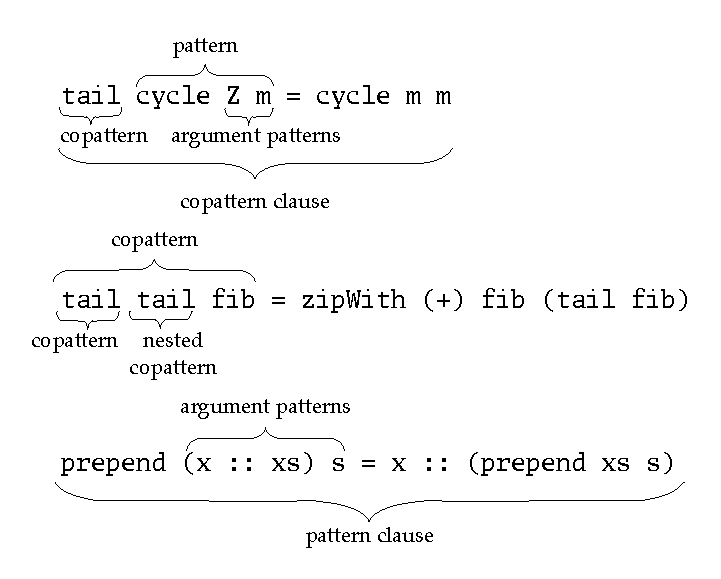
\includegraphics[scale=1]{figures/copattern_anatomy}
  \caption{The anatomy of copatterns.}
  \label{fig:copatterns_anatomy}
\end{figure}

\subsection{Existing Implementations of Copatterns}
Copatterns have already been implemented in other programming languages, for example in
Agda\,\cite{Norell:thesis}. Here, a coinductive type is defined as a record type with a
\texttt{coinductive} flag, an example of which can be seen in
Figure~\ref{fig:agda_stream}. Observations are defined as fields of the record
type, and definitions with copatterns are almost identical to what has already been
discussed. A simple example of a function \texttt{repeat} is given in Figure~\ref{fig:agda_repeat}. 
\begin{figure}[h]
\begin{lstlisting}[mathescape]
record Stream (A : Set) : Set where
  coinductive
  field
    head : A
    tail : Stream A
open Stream
\end{lstlisting}
\caption{\texttt{Stream} definition in Agda.}
\label{fig:agda_stream}
\end{figure}

\begin{figure}[h]
\begin{lstlisting}[mathescape]
repeat : {A : Set} -> A -> Stream A
head (repeat a) = a
tail (repeat a) = repeat a 
\end{lstlisting}
\caption{A corecursive \texttt{repeat} function in Agda.}
\label{fig:agda_repeat}
\end{figure}

In Chapter~\ref{cha:motivation}, we discuss the motivation behind the
use of copatterns. Later, in Chapter~\ref{sec:adding_copatterns}, we describe
our implementation of copatterns in Idris. The implemented
syntax for copatterns involves a prefix character, \texttt{\&}, on the
observation patterns, as pictured in
Figure~\ref{fig:map_copat_syntax}. In the remainder of the report, we will use this
syntax for copattern definitions.

\begin{figure}[h]
\begin{lstlisting}[mathescape]
map : (a -> b) -> Stream a -> Stream b
&head (map f s) = f (head s)
&tail (map f s) = map f (tail s)
\end{lstlisting}
\caption{The \texttt{map} function defined with copatterns using the syntax
  described in Chapter~\ref{sec:adding_copatterns}.}
\label{fig:map_copat_syntax}
\end{figure}

%%% Local Variables: 
%%% mode: latex
%%% TeX-master: "../../copatterns-thesis"
%%% End: 
